

\chapter{Resultados obtenidos}\label{cap:cap5}

A continuación, se detallarán los pasos realizados para el diseño y desarrollo de la aplicación, teniendo en cuenta los requisitos del proyecto y las historias de usuario definidas previamente. Se dividirá la explicación en varias secciones generales, cada una abordando un aspecto clave del proceso de desarrollo:


\begin{itemize}
    \item \textbf{Vistas de la aplicación.}
    
    \item \textbf{Uso de la aplicación.}
    
    \item \textbf{APIs utilizadas.}

    \item \textbf{Aspectos destacables de programación.}

    \item \textbf{Despliegue en entorno de producción.}

    \item \textbf{Costes del proyecto.}
    
\end{itemize}


Cada una de estas secciones será tratada en profundidad en las siguientes subsecciones, proporcionando un análisis detallado de la información correspondiente a cada tema.

\section{Vistas de la aplicación}\label{sec:apartado}

Los modelos de las vistas de la \textcolor{naranja}{sección 4.2 - Modelos para la interfaz - Mockup}
 funcionan como una referencia tanto para el desarrollador como para el cliente, permitiendo una primera aproximación visual de lo que será la aplicación. 

\vspace{0.5cm}

A continuación, se presentan las vistas finales de la aplicación, que han sufrido pocas modificaciones respecto a los modelos iniciales. Además, se describirán de manera general las funcionalidades principales de estas vistas, mientras que el detalle completo se abordará en la  \textcolor{naranja}{sección 5.2 - Uso de la aplicación}.

\vspace{0.5cm}
Procederemos a diferenciar las vistas en cuatro secciones: las destinadas al cliente, las correspondientes al administrador, la vista de la ubicación y la vista responsive, que muestra cómo se adapta la interfaz en dispositivos móviles.

\subsection{Vista para el cliente}\label{subsec5.1.1}

\subsubsection{Login y registro}\label{subsec5.1.1.1}


La vista de login está diseñada para proporcionar una interfaz simple y clara donde los usuarios pueden introducir sus credenciales (correo electrónico y contraseña) para acceder a su cuenta. La estructura visual de esta vista es minimalista, destacando el formulario de autenticación en el centro de la página. Se incluyen campos de texto para el correo electrónico y la contraseña, esta última oculta por defecto para garantizar la seguridad, aunque los usuarios pueden optar por mostrarla utilizando un botón específico. Junto a estos campos, se encuentran botones claramente etiquetados para iniciar sesión (login) y registrarse en caso de no tener cuenta. La vista también ofrece mensajes de error en caso de que los intentos de autenticación sean fallidos.

\begin{figure}[H]
\begin{center}
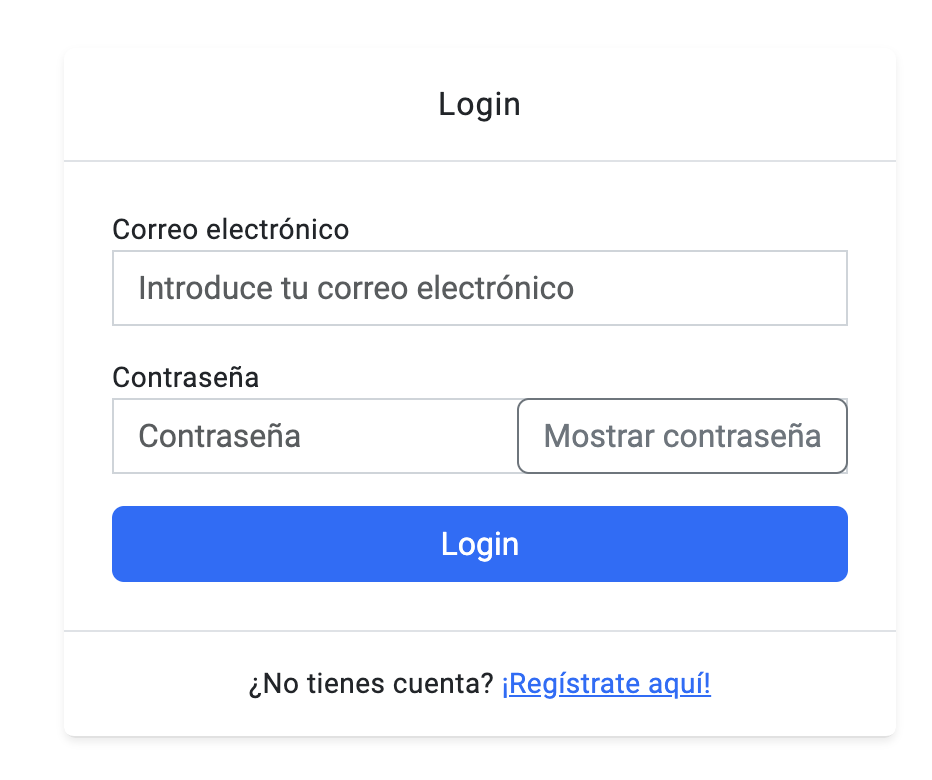
\includegraphics[scale=0.5]{./Images/vista_login.png}
\caption{Vista login} Fuente: Elaboración propia.

\label{fig:fig1}

\end{center}
\end{figure}

La vista de registro presenta un formulario que permite a los nuevos usuarios crear una cuenta en la plataforma. Esta vista está diseñada para ser intuitiva, con campos claramente etiquetados que guían al usuario a través del proceso de registro. Los campos incluyen información básica como nombre y apellidos, identificación, dirección de correo electrónico, y contraseña, además de campos para la dirección. El diseño prioriza la usabilidad y la seguridad, con elementos visuales que validan la información en tiempo real y aseguran que el proceso de registro sea lo más fluido posible.

\begin{figure}[H]
\begin{center}
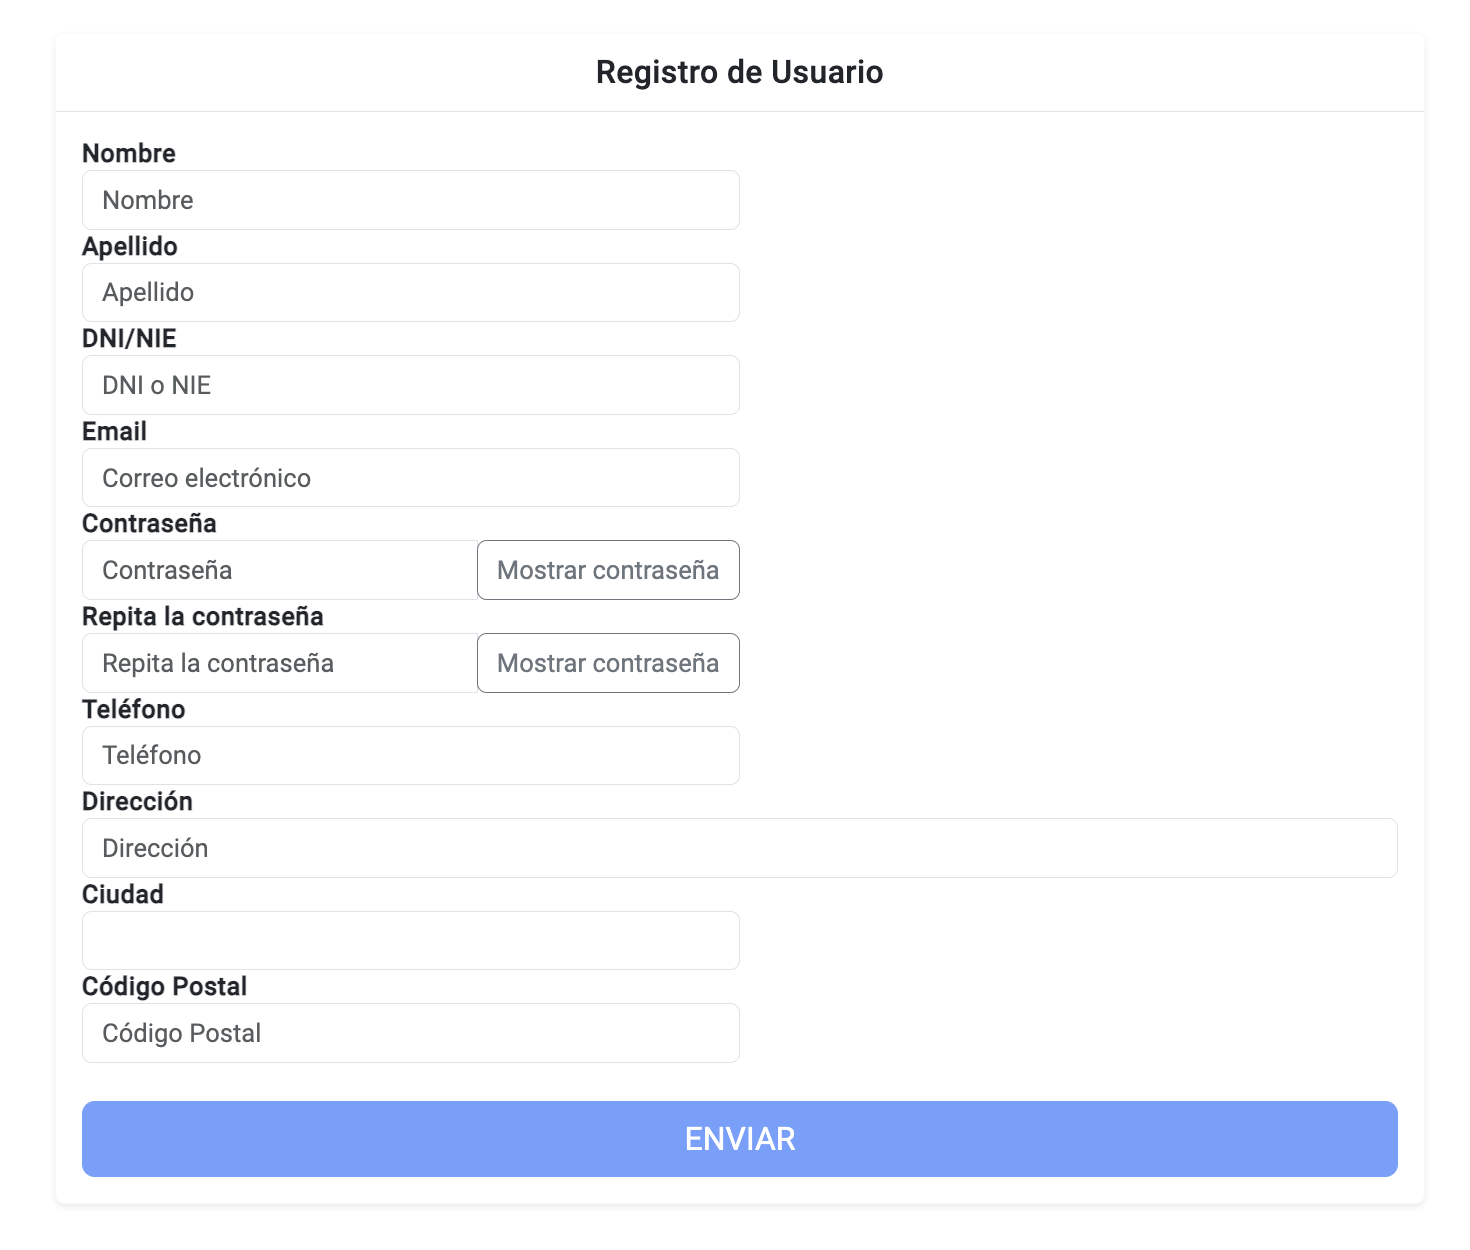
\includegraphics[scale=0.5]{./Images/vista_registro.png}
\caption{Vista registro de usuario} Fuente: Elaboración propia.

\label{fig:fig2}

\end{center}
\end{figure}

\subsubsection{Productos y pedidos}\label{subsec5.1.1.2}

En la vista de productos, se muestran todos los artículos dentro de la categoría seleccionada. Cada producto se presenta con su imagen, nombre, subcategoría, y precio. Además, se incluye una etiqueta informativa que indica si el producto está en oferta, agotado o si forma parte de las últimas novedades

\begin{figure}[H]
\begin{center}
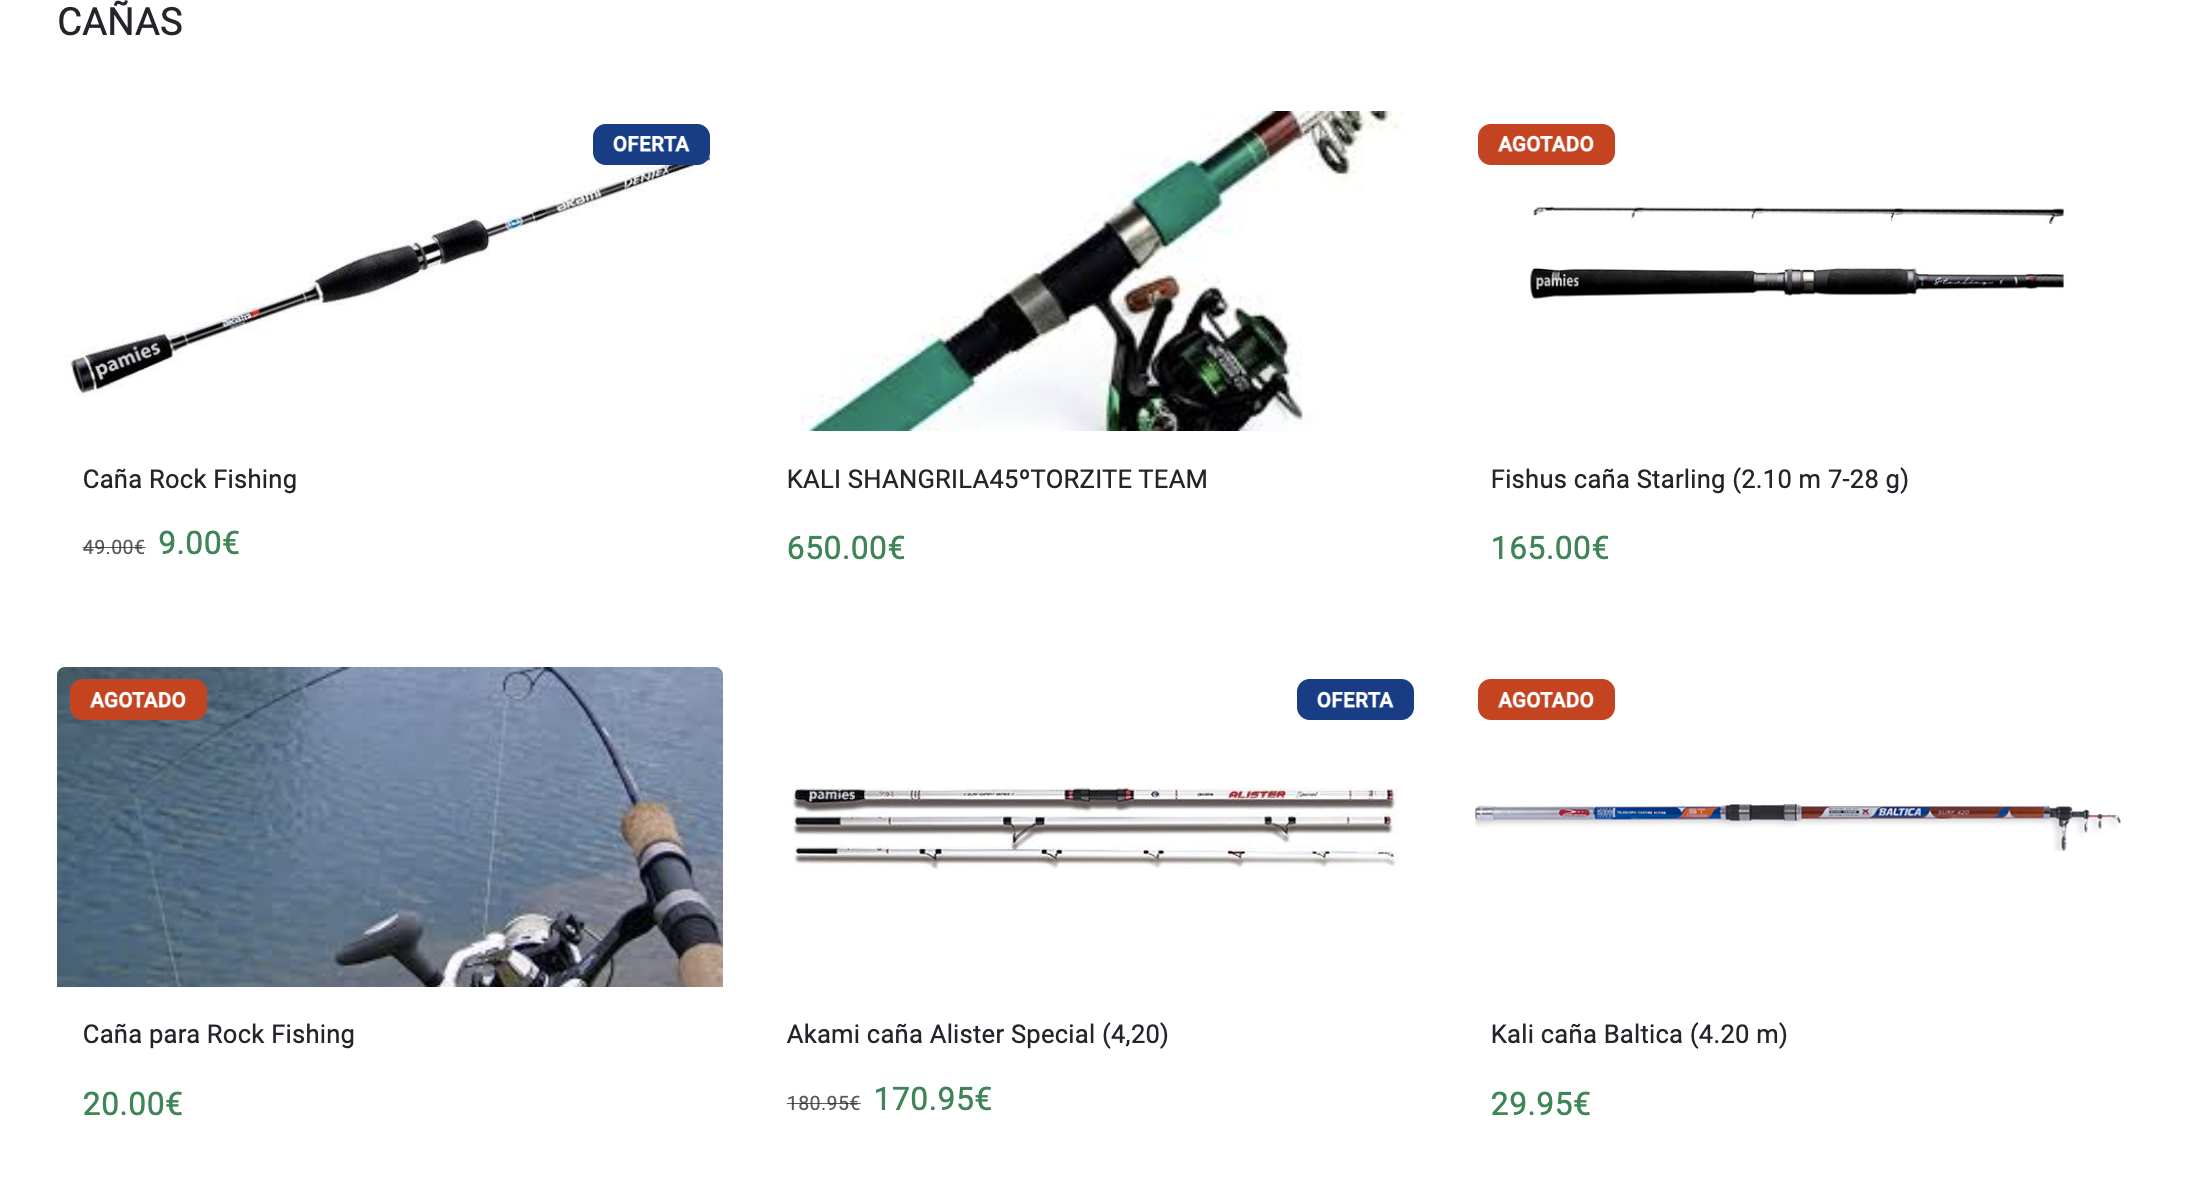
\includegraphics[scale=0.40]{./Images/vistaProductos.png}
\caption{Vista Productos} Fuente: Elaboración propia.

\label{fig:fig2}

\end{center}
\end{figure}


La aplicación también ofrece una vista detallada para cada producto, accesible desde la lista de productos clasificados. En esta vista, los usuarios pueden ver una descripción completa del producto, que incluye información detallada sobre sus características y especificaciones. Además, se muestran múltiples imágenes del producto desde diferentes ángulos, lo que permite a los usuarios examinarlo con mayor precisión. El precio del producto está claramente indicado junto a un botón destacado que permite añadirlo al carrito de compras. También se incluye un campo donde los usuarios pueden especificar la cantidad deseada del producto antes de añadirlo al carrito. Esta vista está diseñada para proporcionar toda la información necesaria para que los usuarios puedan tomar decisiones de compra informadas, al tiempo que facilita el proceso de añadir productos al carrito en las cantidades deseadas.


\begin{figure}[H]
\begin{center}
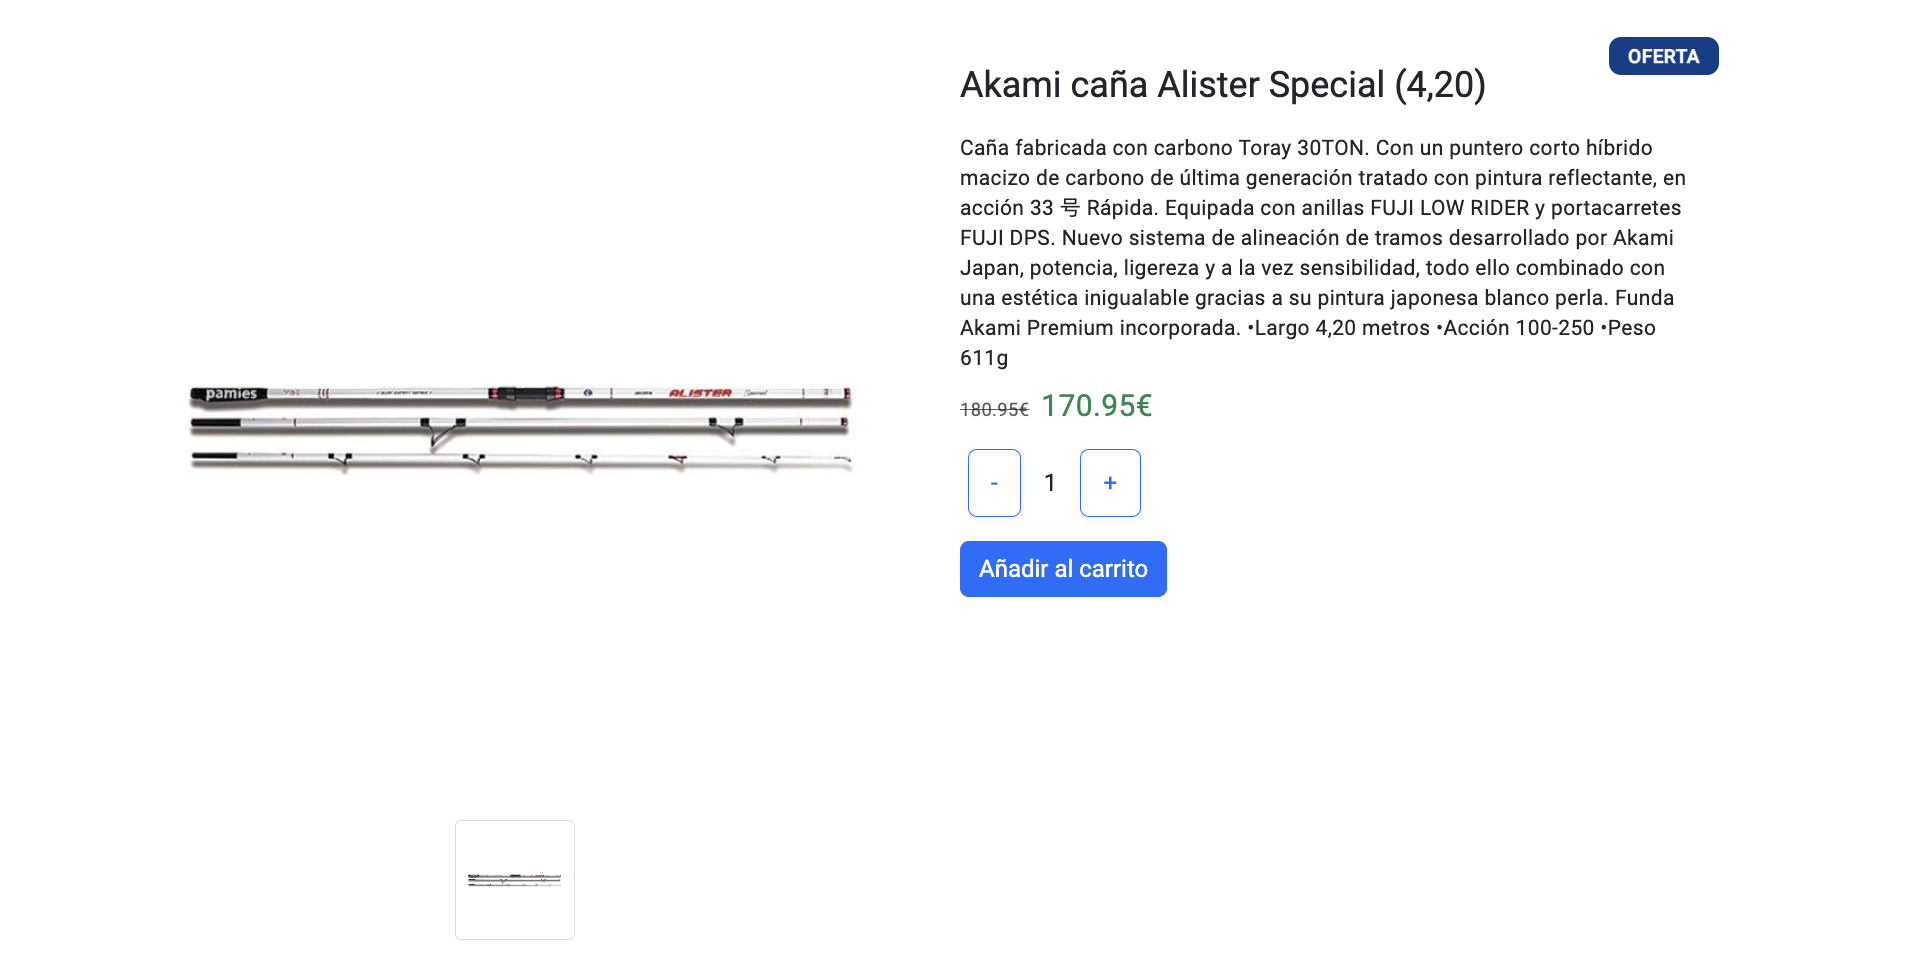
\includegraphics[scale=0.5]{./Images/vistaDetalleProducto.png}
\caption{Vista Detalle de producto} Fuente: Elaboración propia.

\label{fig:fig1}

\end{center}
\end{figure}

A medida que el cliente añade productos, estos se reflejan automáticamente en la vista del carrito. En esta sección se muestra un resumen detallado del pedido, donde es posible visualizar los productos seleccionados, modificar las cantidades o eliminarlos si es necesario. En la parte derecha, se presenta el precio total del pedido junto con un campo donde se puede introducir un código de descuento. Para finalizar, se incluye el botón de 'pagar' que permite al cliente proceder con la confirmación del pedido.


\begin{figure}[H]
\begin{center}
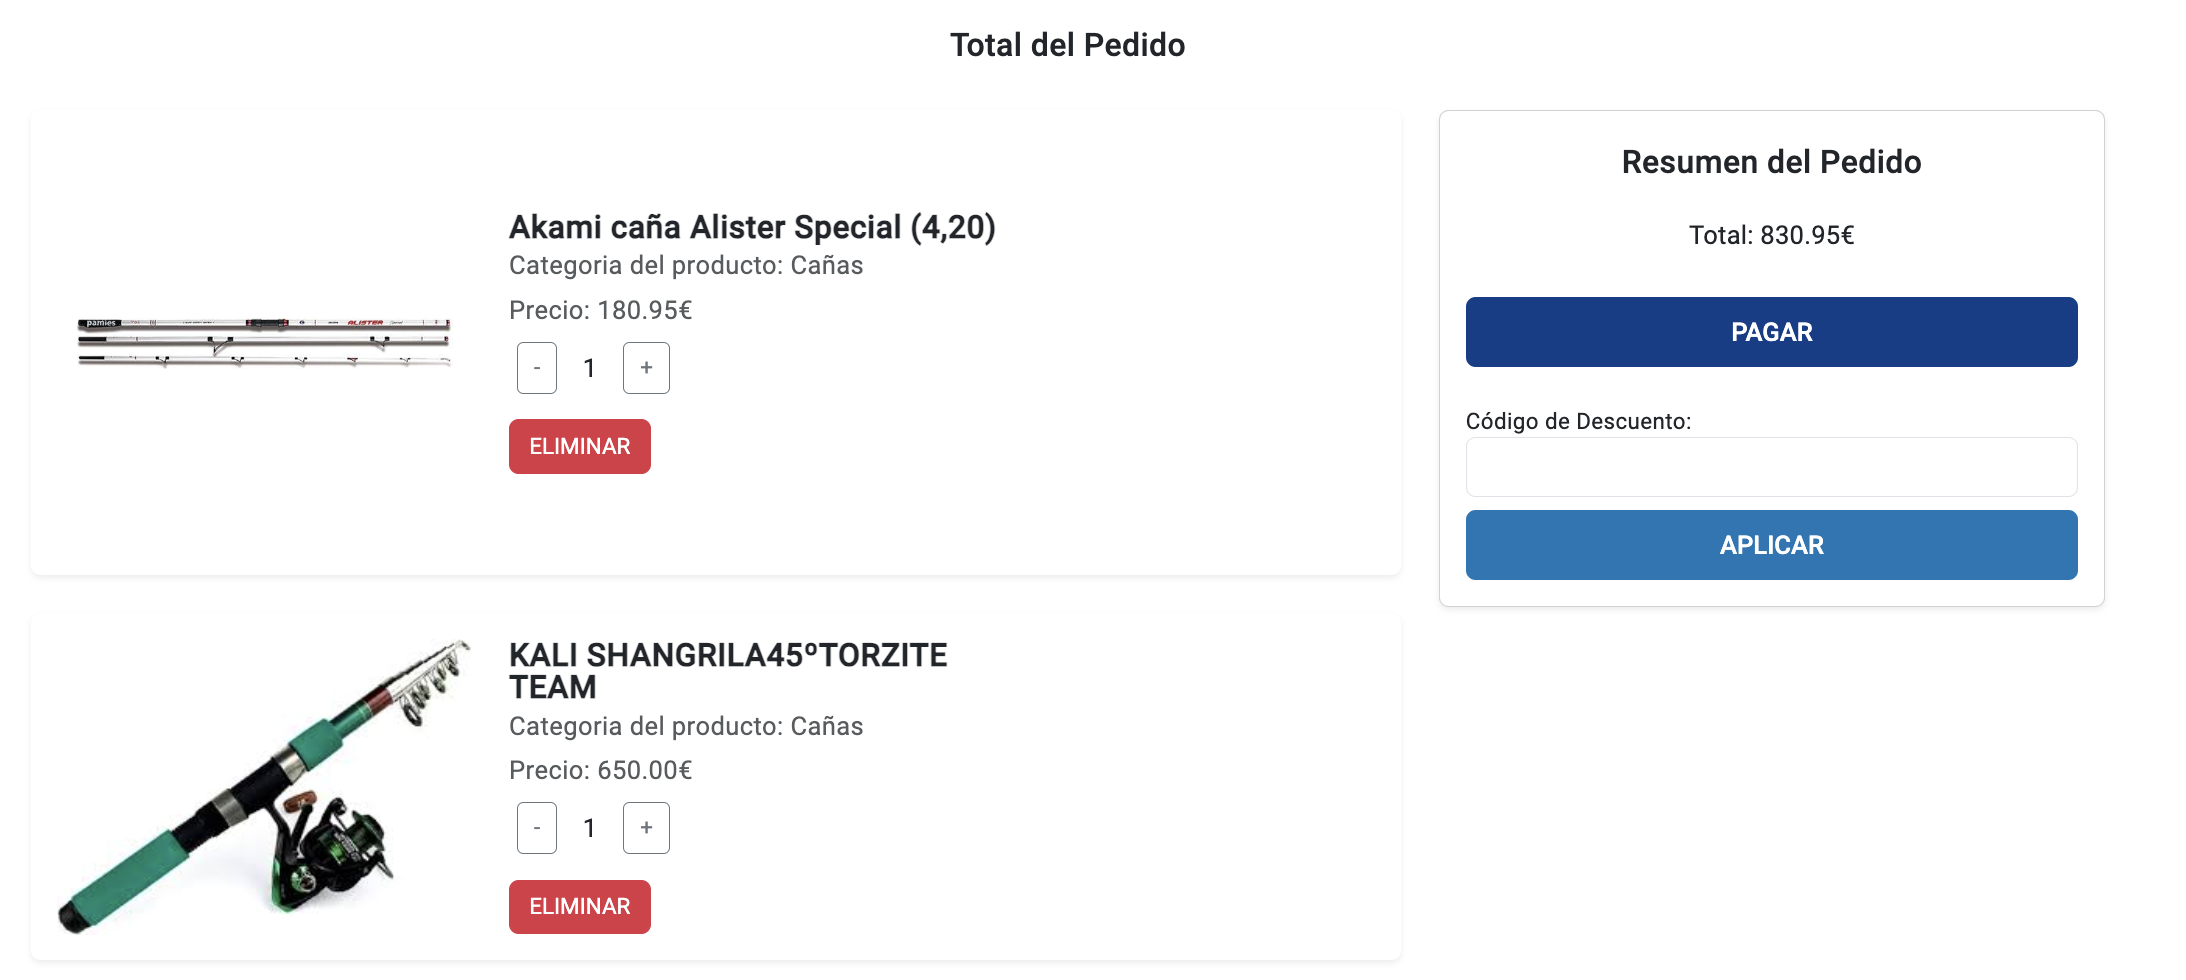
\includegraphics[scale=0.38]{./Images/vistaCarrito.png}
\caption{Vista Carrito de productos} Fuente: Elaboración propia.

\label{fig:fig1}

\end{center}
\end{figure}

Una vez que el cliente confirma el pedido, se genera una pantalla de confirmación en la que se muestra el número de pedido, los productos adquiridos con sus respectivas cantidades y precios, y el total del pedido. Esta misma confirmación es enviada por correo electrónico al cliente para su registro.

\begin{figure}[H]
\begin{center}
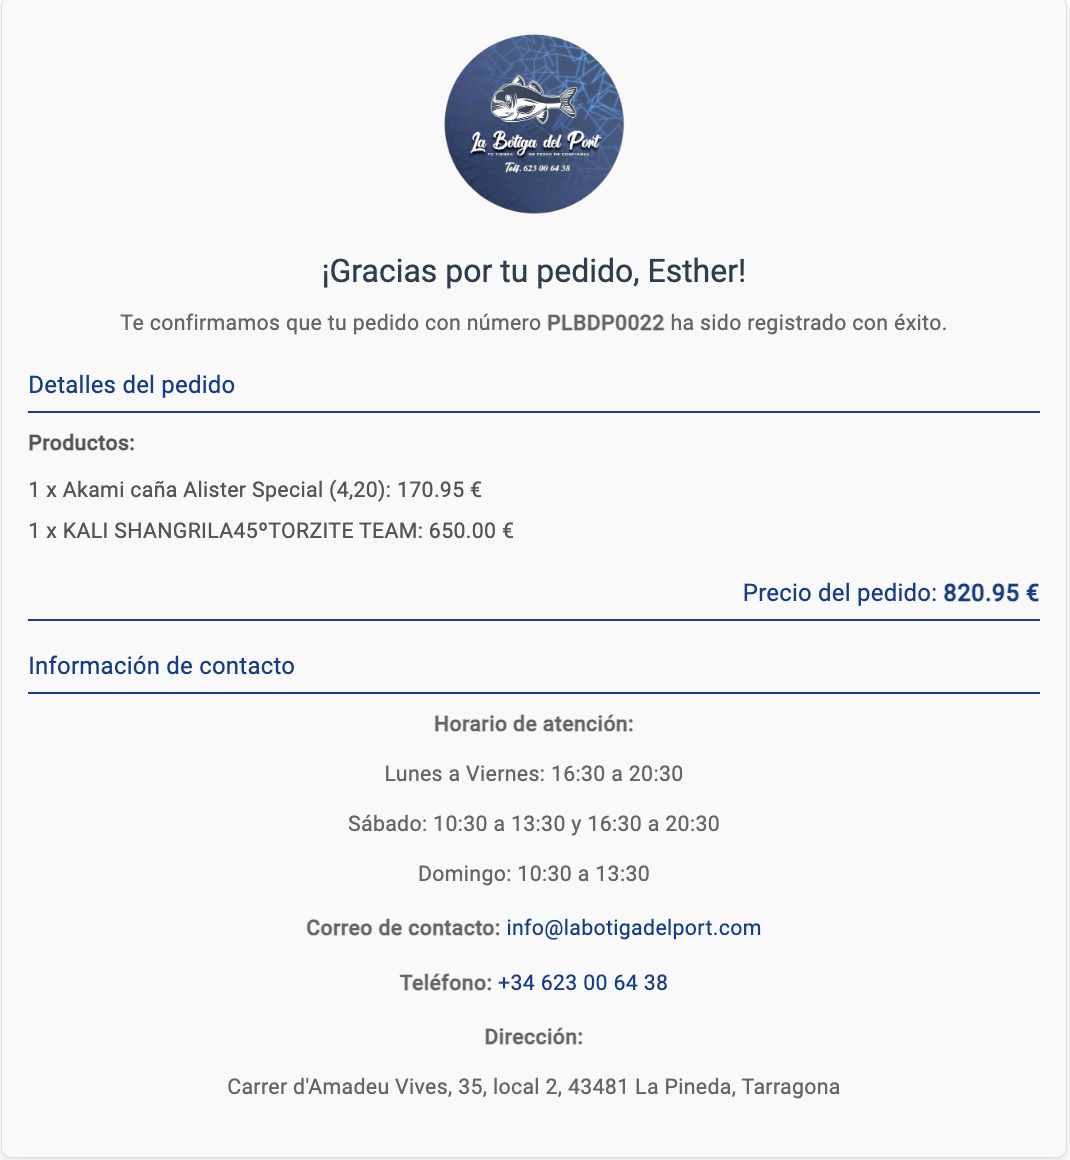
\includegraphics[scale=0.5]{./Images/vistaConfirmacionPedido.png}
\caption{Vista Confirmación del pedido} Fuente: Elaboración propia.

\label{fig:fig1}

\end{center}
\end{figure}

El cliente tiene la opción de ver todos los pedidos que ha realizado en la sección de "Perfil". En este apartado, además de visualizar sus datos personales, puede acceder al historial completo de sus compras, incluyendo detalles de cada pedido, como productos adquiridos, cantidades, precios y fechas. Esto le permite llevar un control de todas sus transacciones a lo largo del tiempo.

\begin{figure}[H]
\begin{center}
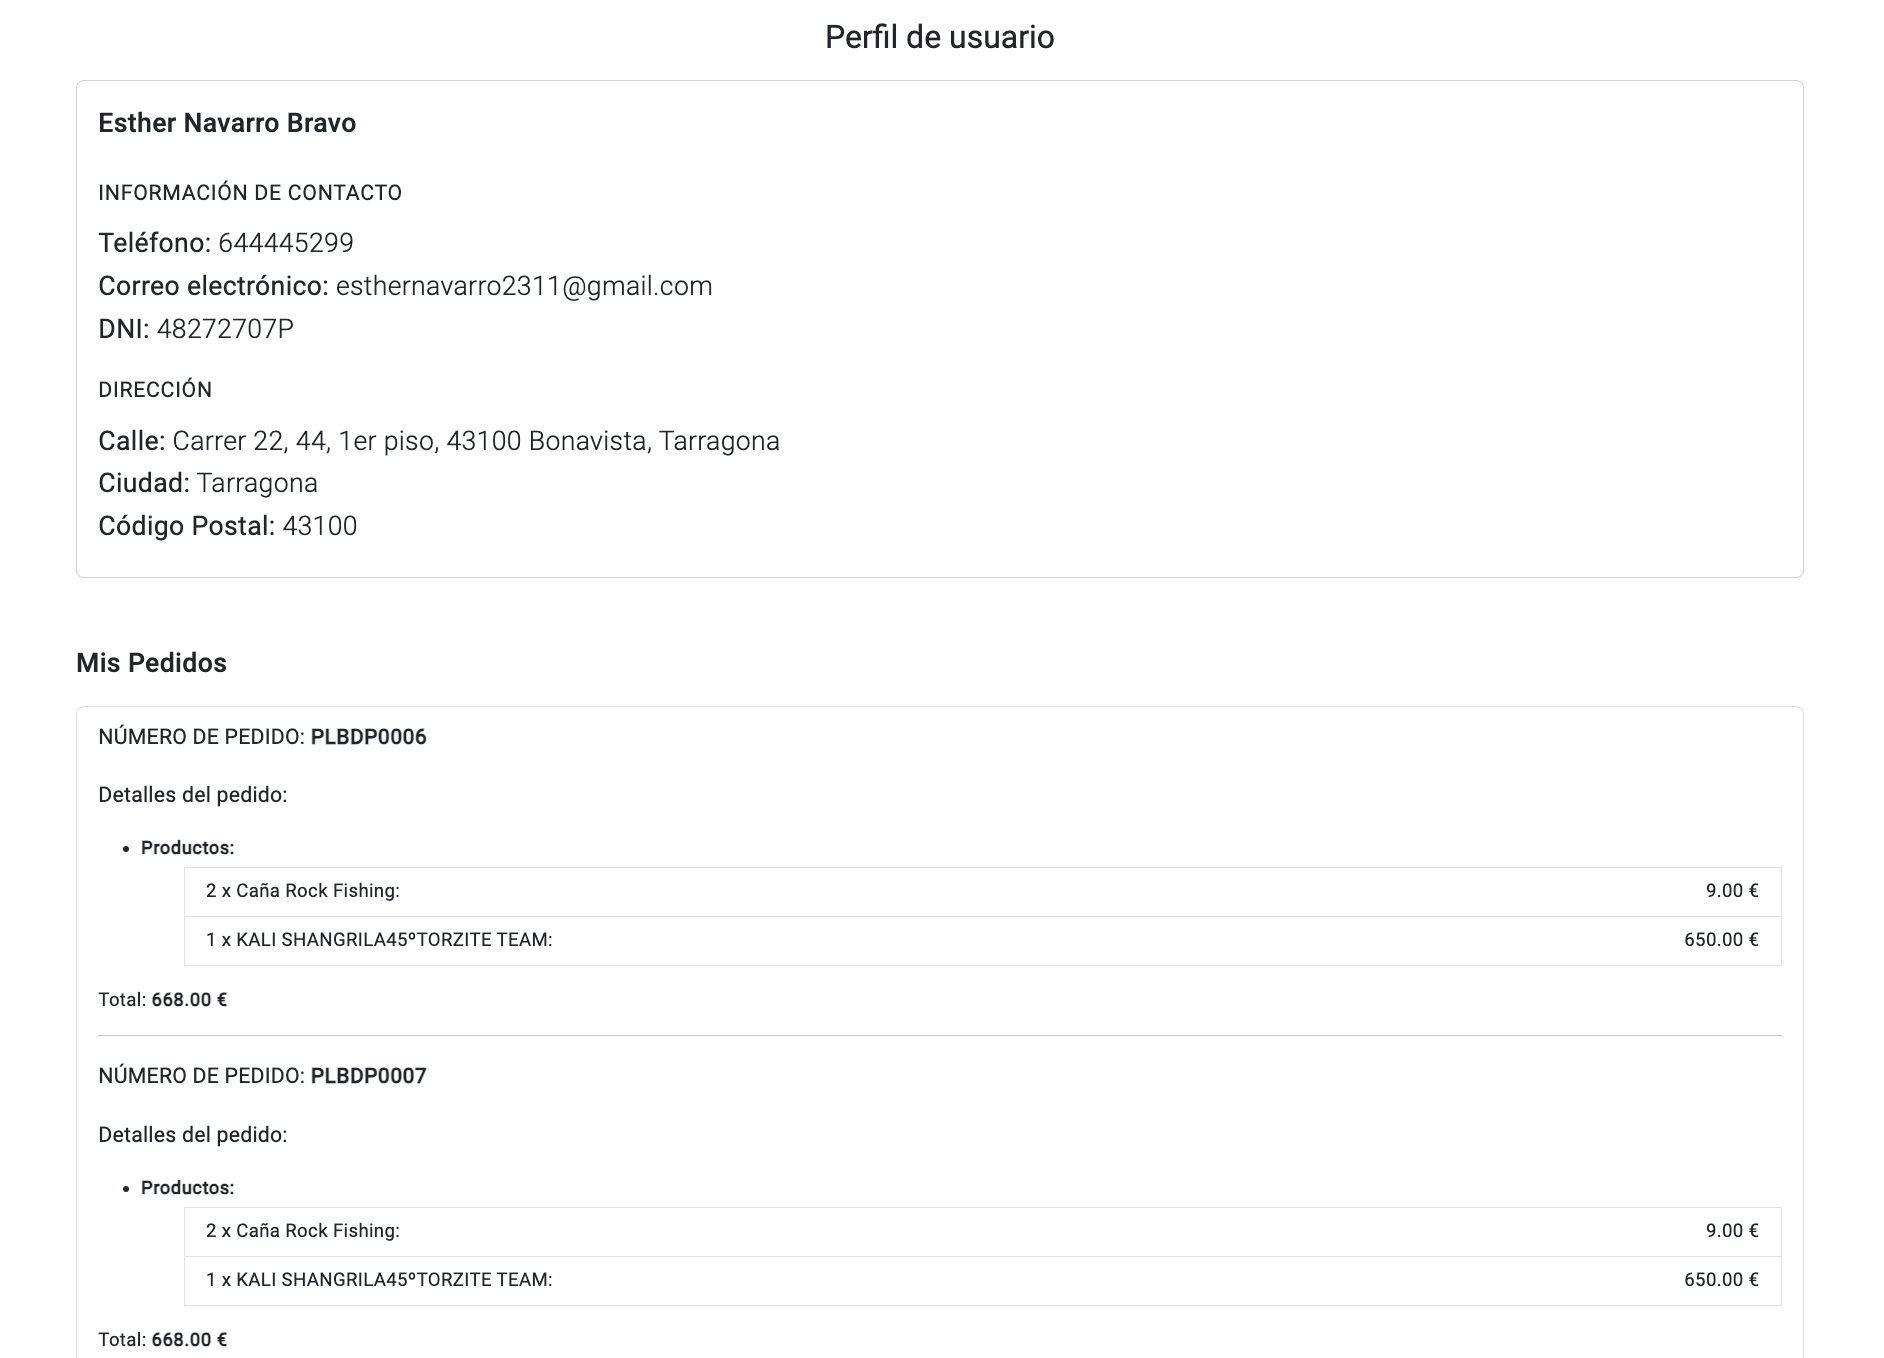
\includegraphics[scale=0.5]{./Images/vistaPerfilUsuario.png}
\caption{Vista Perfil del cliente} Fuente: Elaboración propia.

\label{fig:fig1}

\end{center}
\end{figure}


\subsubsection{Reserva de cebo}\label{subsec5.1.1.3}

La vista de Reserva de cebo permite a los usuarios seleccionar productos relacionados con el cebo de pesca de manera sencilla. Cada producto se muestra con su nombre, imagen representativa y precio. El usuario tiene la opción de elegir la cantidad de cada producto que desea adquirir y debe seleccionar una fecha de recogida antes de proceder. Esta interfaz asegura que toda la información relevante esté fácilmente accesible, facilitando la navegación y el proceso de reserva.

\begin{figure}[H]
\begin{center}
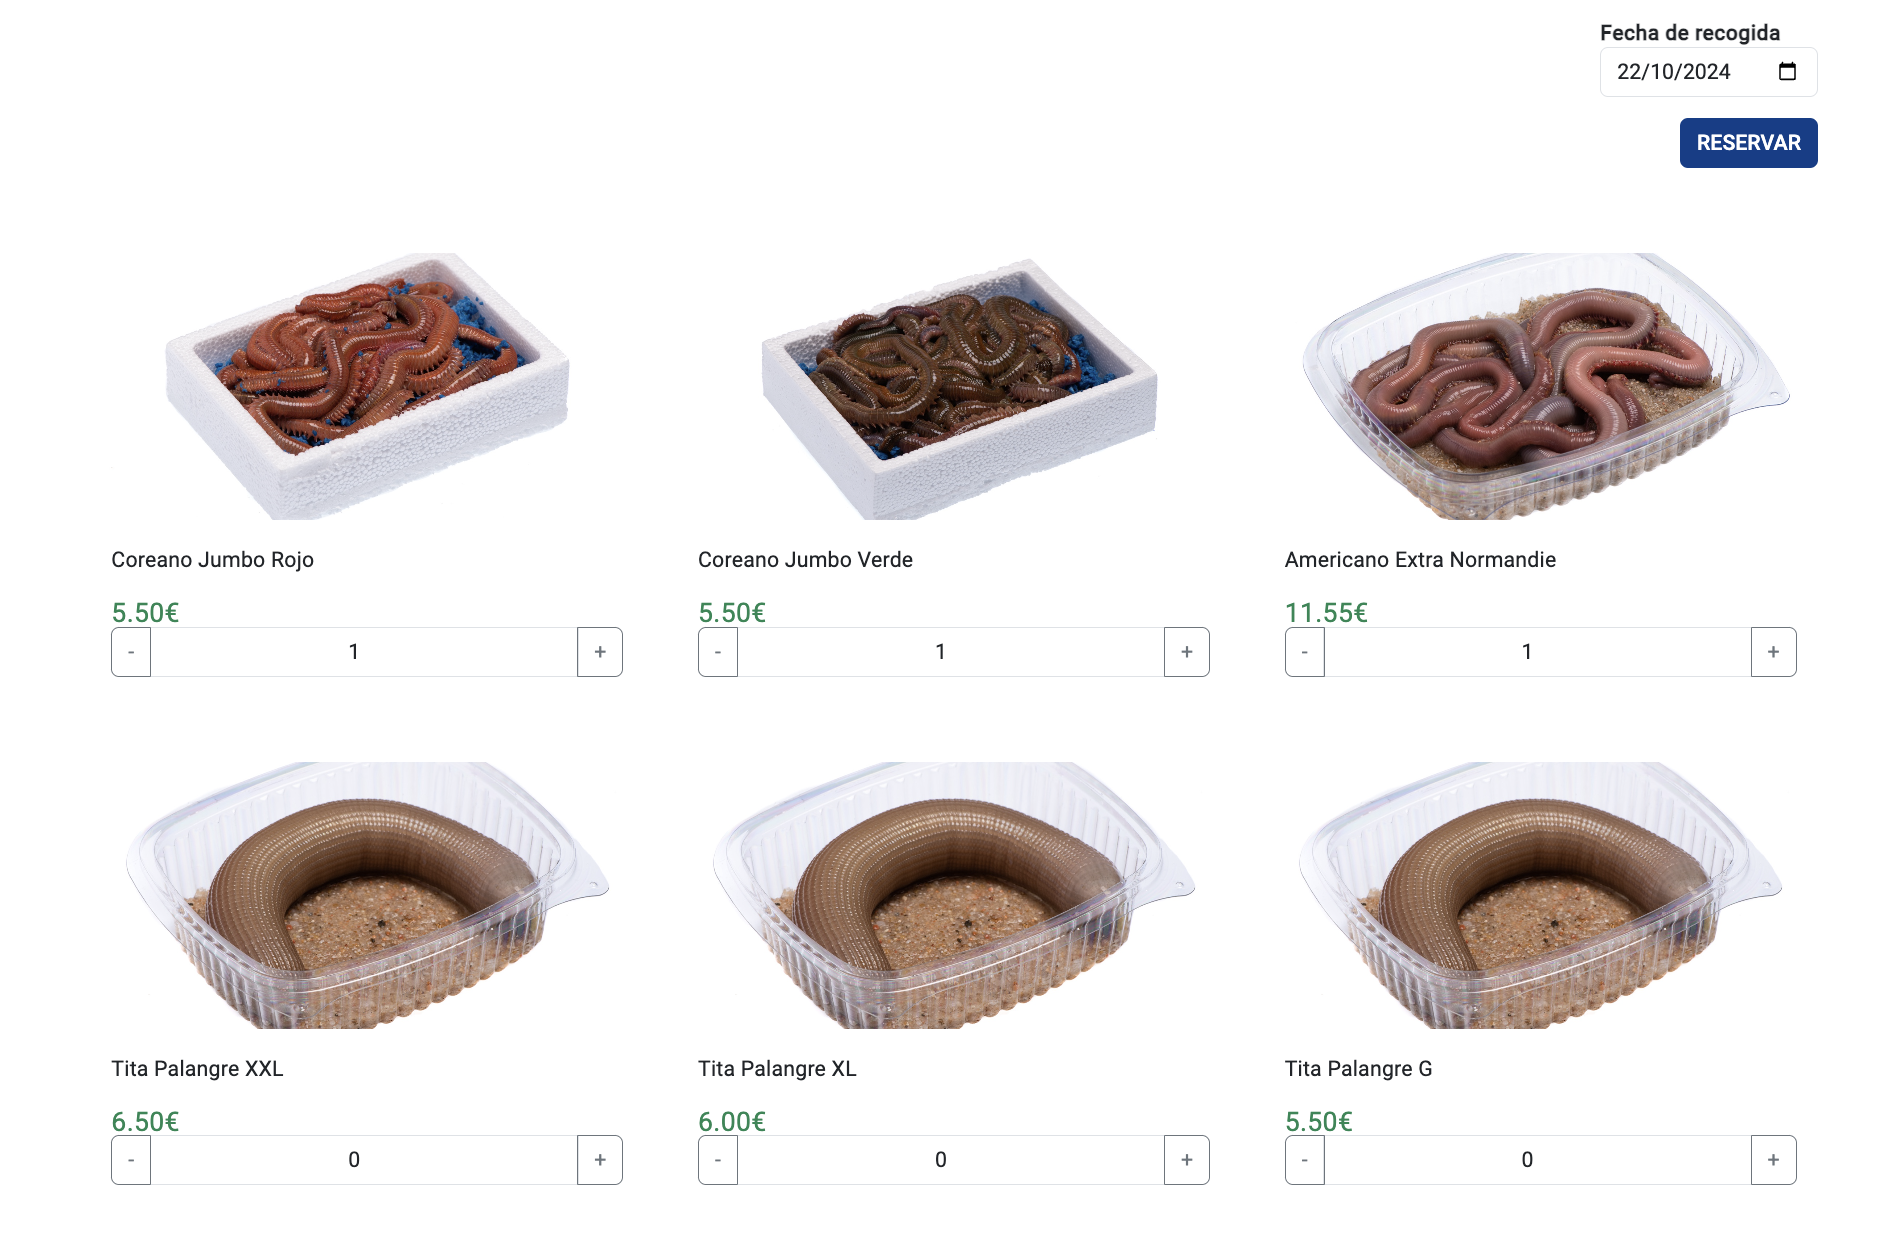
\includegraphics[scale=0.5]{./Images/vistaReservaCebo.png}
\caption{Vista Reserva de cebo} Fuente: Elaboración propia.

\label{fig:fig1}

\end{center}
\end{figure}

Una vez seleccionados los productos, la vista presenta un resumen de la reserva, en el que se detalla cada artículo, incluyendo las cantidades elegidas. Desde esta sección, los usuarios pueden ajustar la cantidad de cada producto si lo consideran necesario. El precio total de la reserva se calcula y se muestra automáticamente, brindando una visión clara del coste final. Cuando el usuario está satisfecho con su selección, puede proceder a confirmar la reserva.

\begin{figure}[H]
\begin{center}
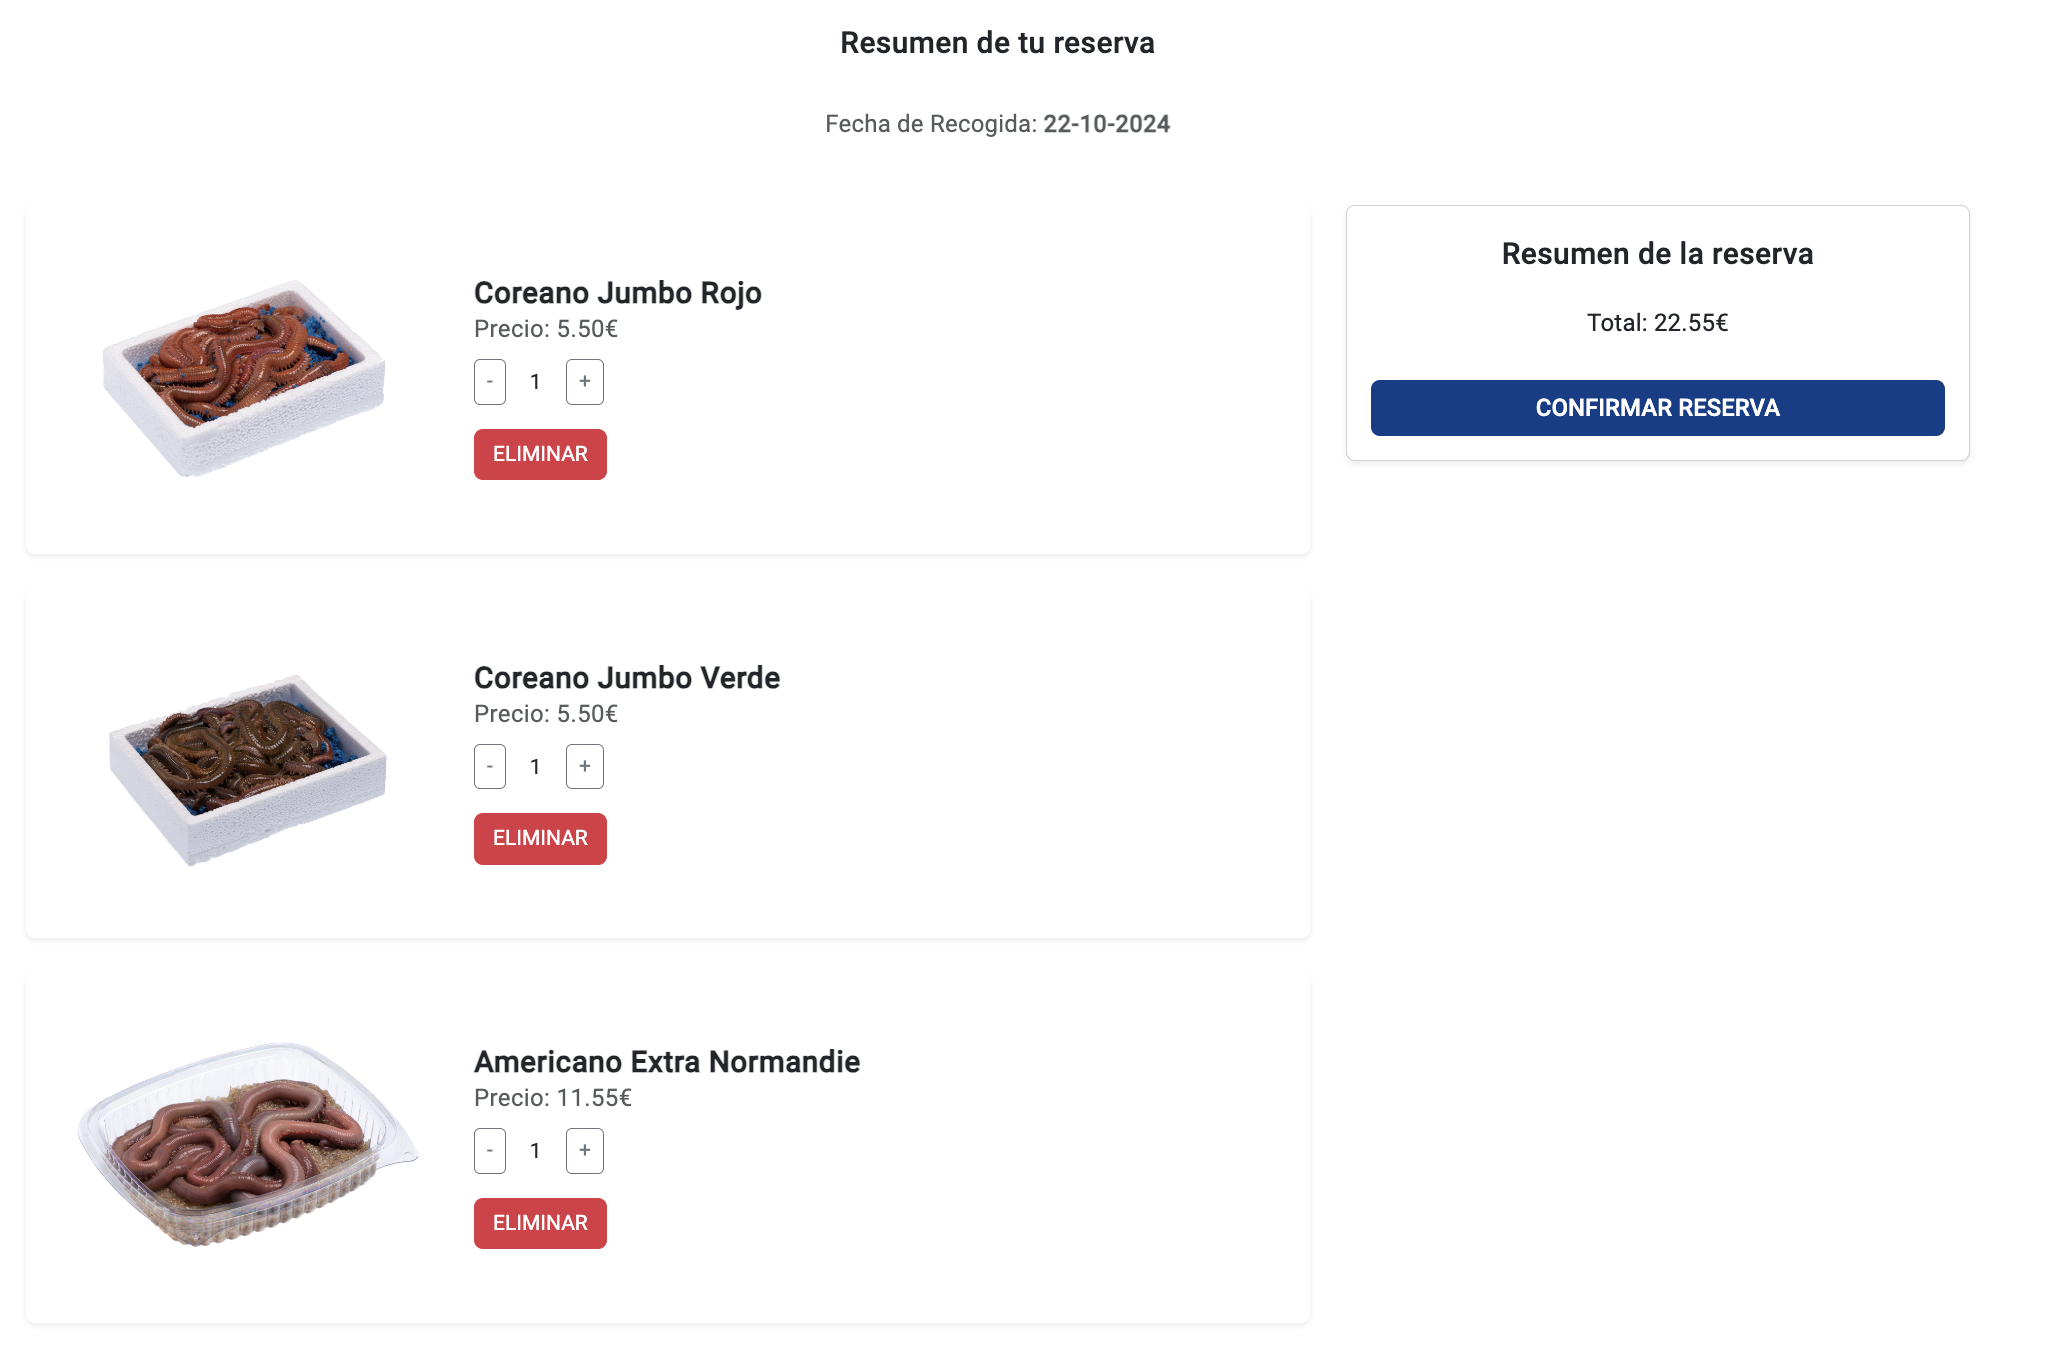
\includegraphics[scale=0.5]{./Images/vistaResumenReservaCebo.png}
\caption{Vista Resumen reserva de cebo} Fuente: Elaboración propia.

\label{fig:fig1}

\end{center}
\end{figure}

Después de confirmar la reserva, el sistema genera un resumen completo de la misma, mostrando los productos seleccionados, la cantidad de cada uno y el precio total. Este resumen se presenta tanto en pantalla como en un correo electrónico que se envía automáticamente al cliente, asegurando que el usuario tenga un registro de su pedido.

\begin{figure}[H]
\begin{center}
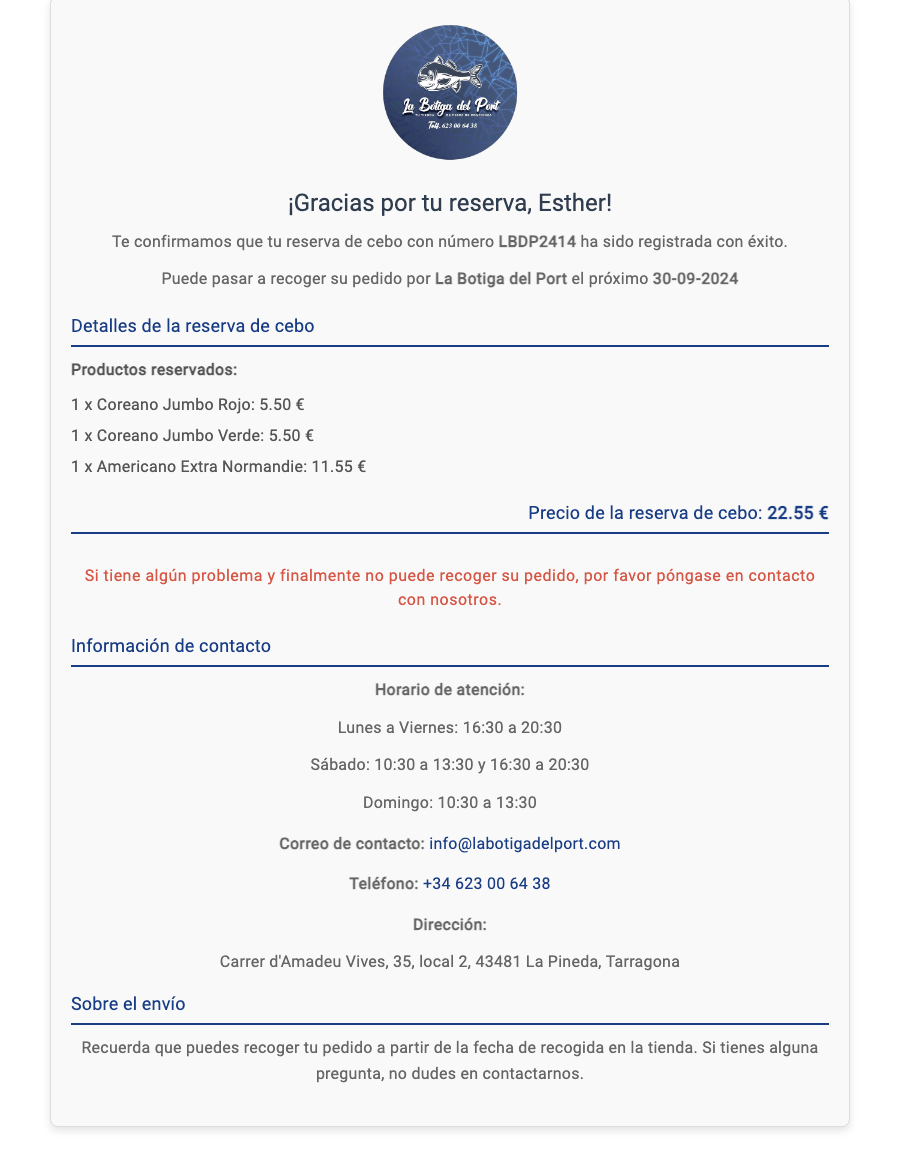
\includegraphics[scale=0.7]{./Images/vistaConfirmacionReservaCebo.png}
\caption{Vista Confirmación reserva de cebo} Fuente: Elaboración propia.

\label{fig:fig1}

\end{center}
\end{figure}

\subsubsection{Página principal}\label{subsec5.1.1.4}

En la página principal, se presentan tres módulos clave para una experiencia de usuario atractiva y funcional. El primer módulo es un banner informativo que incluye un título, un subtítulo y un botón que dirige al cliente a una página o enlace específico. Este banner es ideal para destacar las promociones vigentes o para redirigir a los usuarios a páginas importantes, como ofertas especiales, lanzamientos de productos o eventos destacados.

\begin{figure}[H]
\begin{center}

\includegraphics[scale=0.4]{./Images/vistaBanner.png}
\caption{Banner informativo} Fuente: Elaboración propia.

\label{fig:fig1}

\end{center}
\end{figure}

El segundo módulo es un carrusel que muestra los seis productos más vendidos de la tienda. Cada producto se presenta con su imagen, nombre y precio, ofreciendo una vista clara y atractiva de los artículos más populares. Al hacer clic en cualquiera de estos productos, el cliente es redirigido a la página de detalles del producto, donde puede obtener más información y realizar la compra.

\begin{figure}[H]
\begin{center}
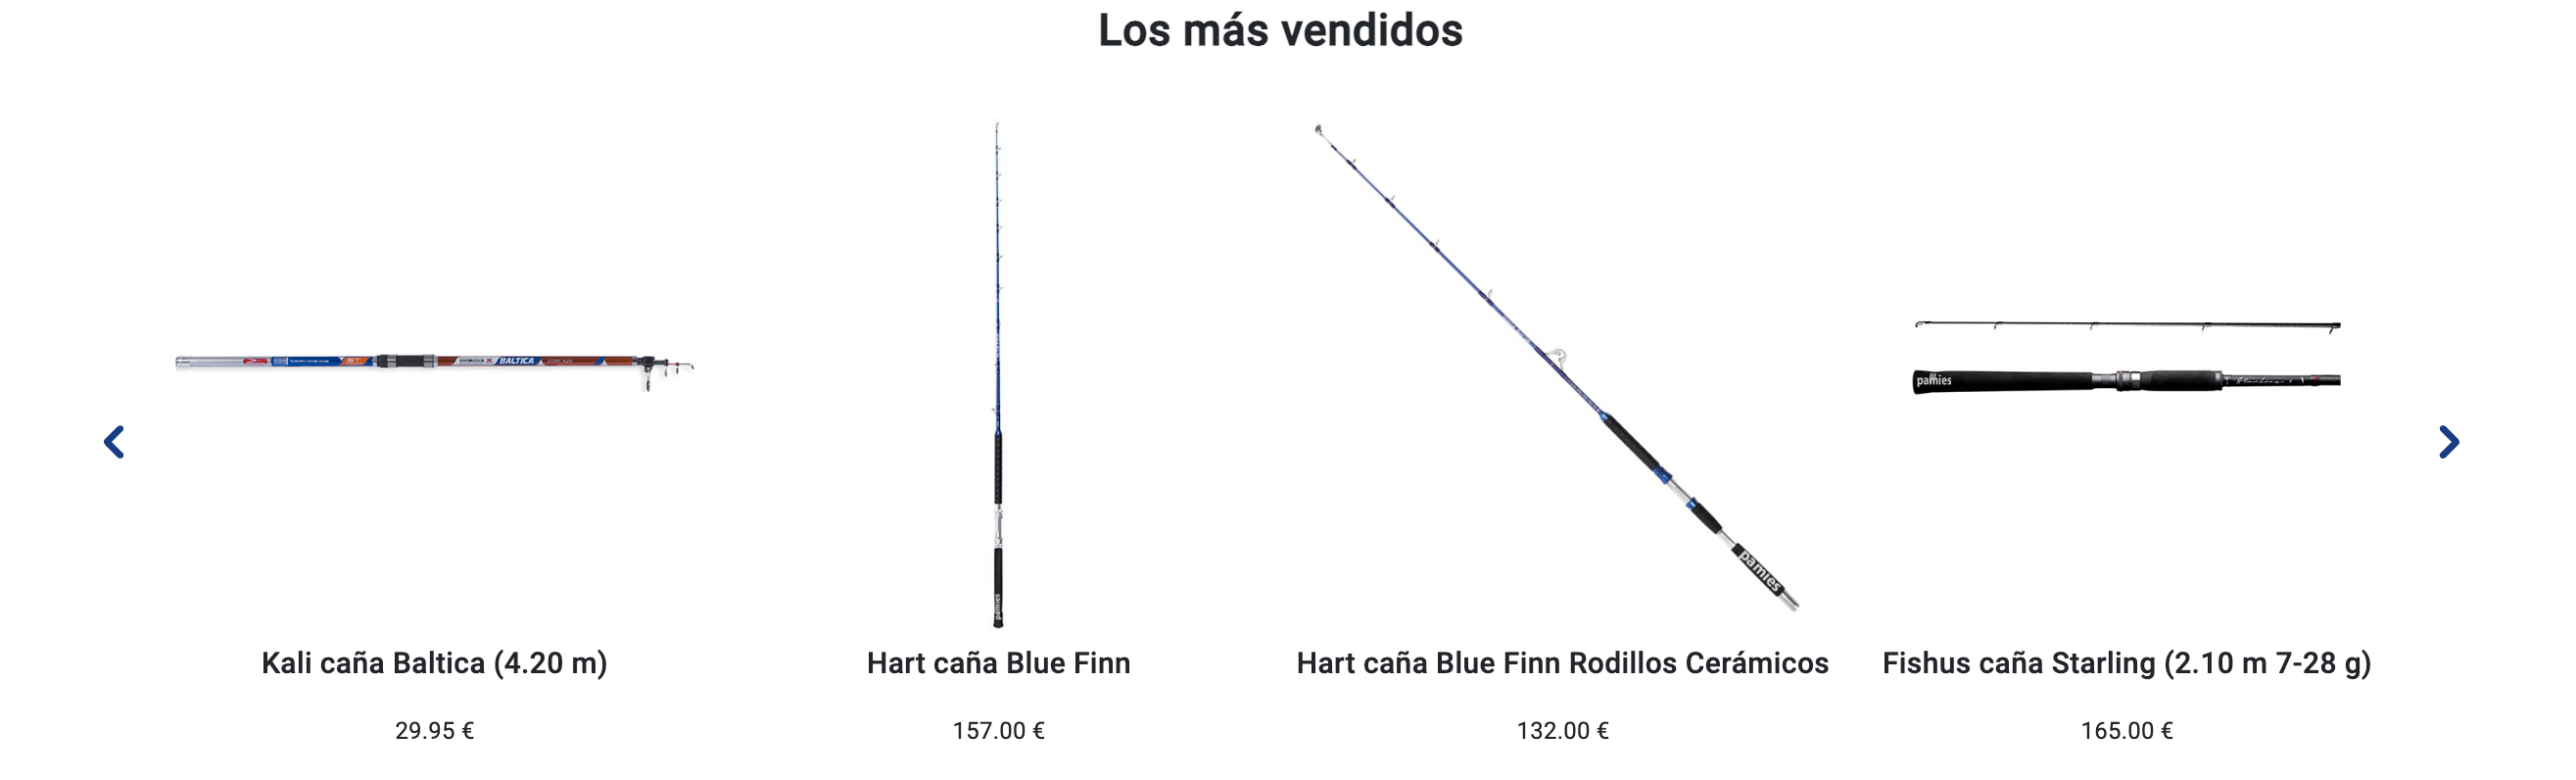
\includegraphics[scale=0.35]{./Images/vistaCarrusel.png}
\caption{Carrusel de productos} Fuente: Elaboración propia.

\label{fig:fig1}

\end{center}
\end{figure}

El tercer módulo consta de tres tarjetas que representan las categorías de novedades, ofertas y liquidaciones. Estas tarjetas permiten un acceso rápido a las páginas específicas de cada categoría, mostrando los productos que cumplen con estas características. Al hacer clic en cada tarjeta, el usuario es dirigido a la página correspondiente, donde podrá explorar los productos disponibles bajo novedades, ofertas o liquidaciones, según su interés.

\begin{figure}[H]
\begin{center}
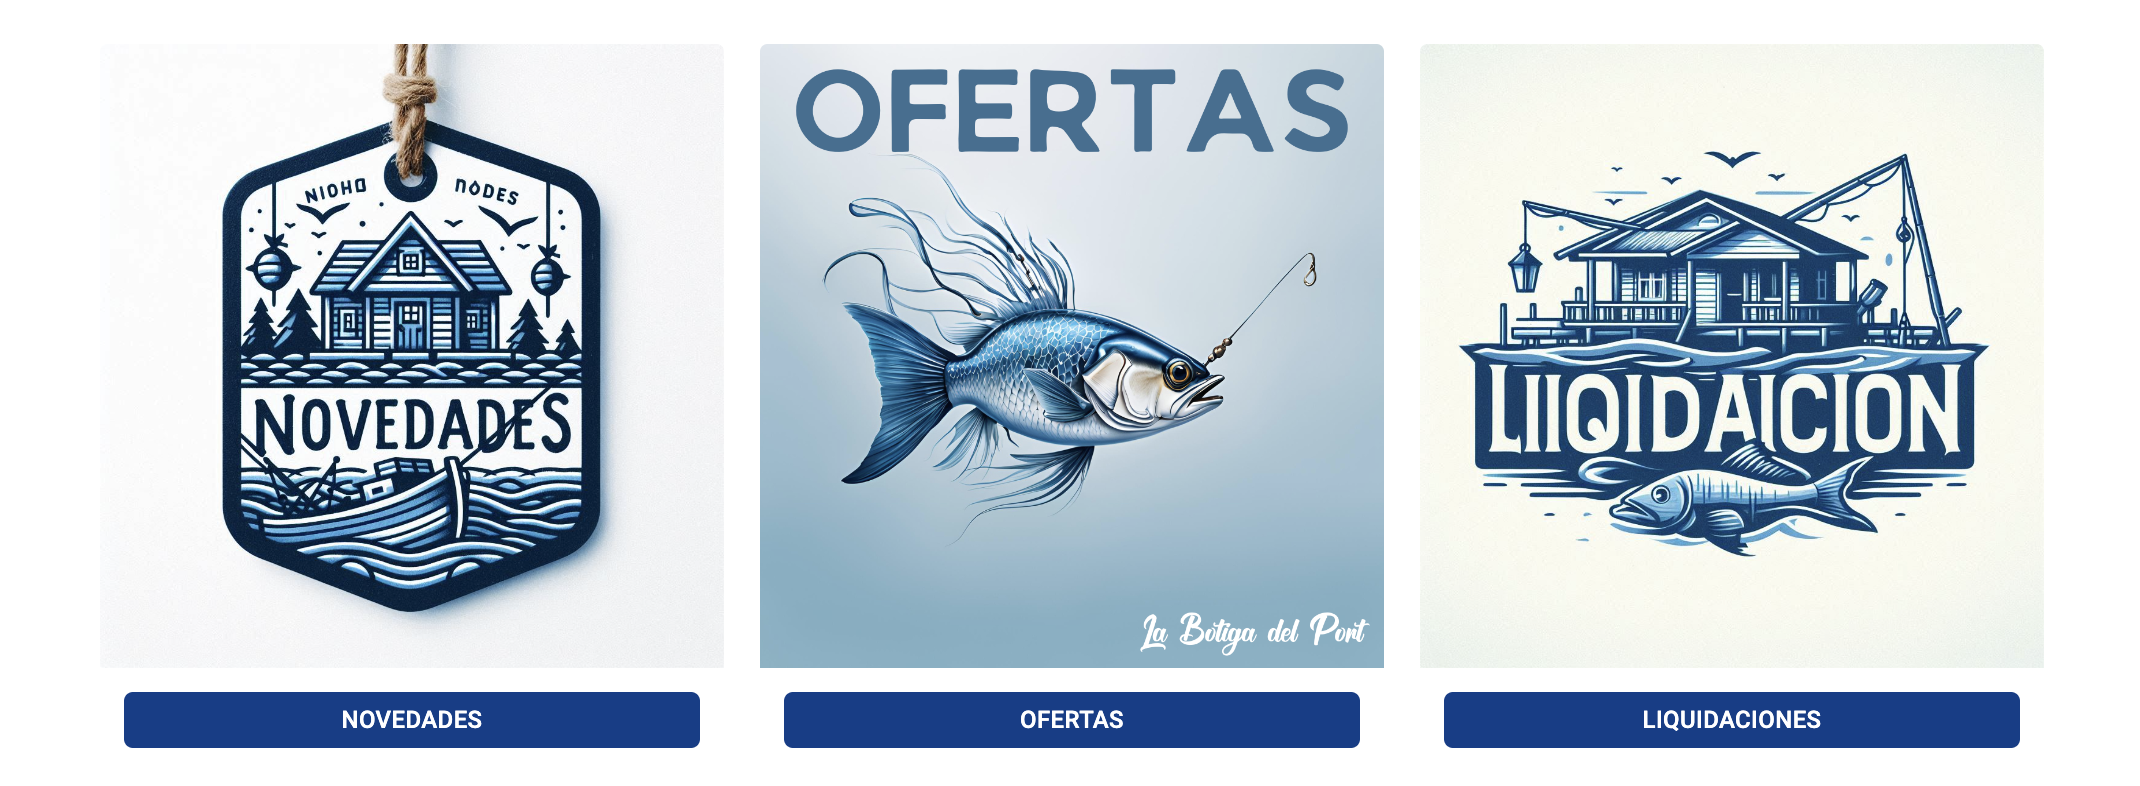
\includegraphics[scale=0.4]{./Images/vistaCards.png}
\caption{Tarjetas de acceso rápido} Fuente: Elaboración propia.

\label{fig:fig1}

\end{center}
\end{figure}


